As mentioned the previous tests learning curves semed to have plateaued. Therefore we will run the configuration from the previous test with seed 0 and the SIGN improvement function with 500 base learning steps. This is to see if the learning did plateau. If that is the case the solver iteration counts should stay relatively unchanged. Or if the algorithm could find a better preconditioner after the base 100 learning steps from the previous test.

What we get from the learning curve in figure \ref{fig: plateau learning curves} is that the learning has plateaued and no significant changes are made after 500th learning step. The fluctuations is inherent to the SIGN improvement function, which has been mentioned earlier. In the evaluation of the learned preconditioner there is no significant differences between the run with 100 and 500 base learning steps, having only slightly higher mean and median solver iteration counts, this is because in the current version of the algorithm the learned preconditioner is the last version in learning, meaning because of the fluctuations it ended in with a slightly worse preconditioner.

\begin{figure}[H]
    \begin{minipage}{.49\textwidth}
        \center
        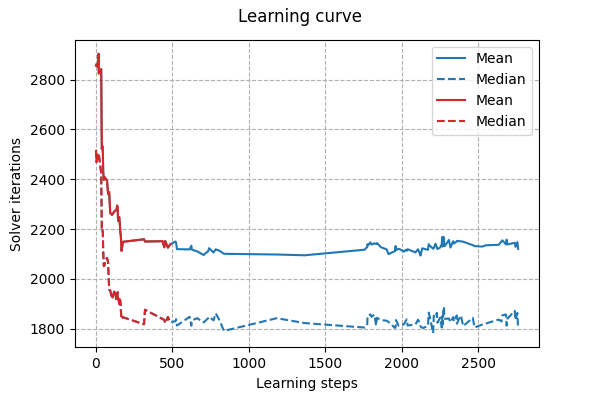
\includegraphics[width=1\textwidth]{plots/plateau_learning_curve.png}
        \caption{Learning curve for seed 0 and SIGN improvement function with 100 base learning iterations, red curve, and 500 base learning iterations, blue curve. Line style indicate mean (full line) and median (dashed line) solver iteration count.}
        \label{fig: plateau learning curves}
    \end{minipage}
    \begin{minipage}{.02\textwidth}
        
    \end{minipage}
    \begin{minipage}{.49\textwidth}
        \center
        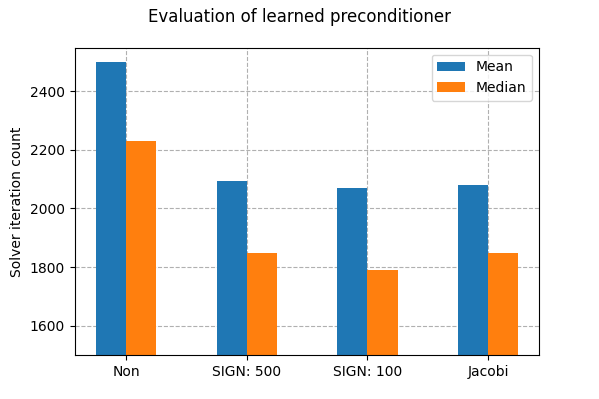
\includegraphics[width=1\textwidth]{plots/plateau_test_measure.png}
        \caption{Evaluation of the learned preconditioner, with the same structure as figure \ref{fig: jacobi par shift test measure}, for the run with seed 0 and SIGN improvement function with 100 and 500 base learning iterations.\\}
        \label{fig: plateau test measure}
    \end{minipage}
\end{figure}